\chapter{Numeryczny rozmyty regulator FGPC--NPL}
\section{Algorytm z predykcją nieliniową}
W części~4 zaimplementowano algorytm FGPC--NPL (materiały wykładowe \emph{Regulatory rozmyte}, s.~168--169, wzory (4.103)--(4.105) oraz (4.118)--(4.125)). Model TS, macierz dynamiczna $M_k$ z linearyzacji w bieżącym $y(k)$ oraz zadanie \texttt{quadprog} z ograniczeniami $0\leq u\leq200$, $|\Delta u|\leq15\ \jednprzep$ pozostają takie same jak w części~3.

Zmienia się sposób wyznaczania odpowiedzi swobodnej $Y^0(k)$. Najpierw wyznacza się błąd modelu $d_k$ z pełnego modelu rozmytego (wzory (4.118)--(4.119)):
\begin{align}
 y^{\mathrm{mod}}(k)&=\sum_{i=1}^5\widetilde w_i\bigl(y(k-1)\bigr)\Bigl(b_{1,i}y(k-1)+b_{2,i}y(k-2)\nonumber\\
 &\qquad+c_{1,i}u(k-11)+c_{2,i}u(k-12)+a_{0,i}\Bigr),\\
 d_k&=y(k)-y^{\mathrm{mod}}(k),
\end{align}
a następnie oblicza kolejne próbki $y^0(k+p|k)$ ($p=1,\dots,N$) iteracyjnie, aktualizując wagi $\widetilde w_i$ w każdym kroku horyzontu (wzory (4.120)--(4.125)):
\begin{align}
 y^0(k+p|k)&=d_k+\sum_{i=1}^5\widetilde w_i\bigl(y^0(k+p-1|k)\bigr)\Bigl(b_{1,i}y^0(k+p-1|k)+b_{2,i}y^0(k+p-2|k)\nonumber\\
 &\qquad+c_{1,i}u^0(k+p-11)+c_{2,i}u^0(k+p-12)+a_{0,i}\Bigr),
\end{align}
dla $y^0(k|k)=y(k)$, $y^0(k-1|k)=y(k-1)$ oraz $u^0(k+j)=u(k-1)$ ($j\geq0$).

\section{Strojenie \texorpdfstring{$\lambda$}{lambda} i porównanie wszystkich regulatorów}
Dla FGPC--NPL użyto tych samych nastaw $N=30$, $N_u=5$ i $\lambda\in\{2;\ 1;\ \num{0.5};\ \num{0.2}\}$ co dla FGPC--SL (por. Przykład~4.19 w materiałach wykładowych). Tab.~\ref{tab:npl-tuning} porównuje wpływ $\lambda$ w obu algorytmach, a tab.~\ref{tab:npl-summary} zbiera wszystkie regulatory z części~1--4.

\begin{table}[H]
\centering
\caption{Wpływ $\lambda$ na jakość regulacji FGPC--SL i FGPC--NPL ($N=30$, $N_u=5$) w czterech próbach.}
\small
\begin{tabular}{crrrrrrrr}\toprule
 & \multicolumn{4}{c}{FGPC--SL} & \multicolumn{4}{c}{FGPC--NPL}\\\cmidrule(lr){2-5}\cmidrule(lr){6-9}
$\lambda$ & IAE zad. & IAE zakł. & Suma IAE & $\sum|\Delta u|$ & IAE zad. & IAE zakł. & Suma IAE & $\sum|\Delta u|$\\\midrule
\num{2.0} & 11963 & 5102 & 17064 & \num{221.6} & 11748 & 4898 & 16646 & \num{235.8}\\
\num{1.0} & 10849 & 3975 & 14823 & \num{272.1} & 10563 & 3963 & 14526 & \num{304.8}\\
\num{0.5} & 10194 & 3366 & 13561 & \num{325.9} &  9851 & 3486 & 13337 & \num{389.5}\\
\num{0.2} &  9633 & 2941 & 12574 & \num{420.4} &  9227 & 3144 & 12371 & \num{523.3}\\\bottomrule
\end{tabular}
\label{tab:npl-tuning}
\end{table}

\begin{table}[H]
\centering
\caption{Zestawienie wszystkich regulatorów z części~1--4 w czterech próbach projektowych.}
\small
\begin{tabular}{lrrrrrrr}\toprule
Regulator & IAE zad. & IAE zakł. & Suma IAE & Przereg. & Cofn. & $\max|e_{F_D}|$ & $\sum|\Delta u|$\\
 & [cm$\cdot$s] & [cm$\cdot$s] & [cm$\cdot$s] & [cm] & [cm] & [cm] & [$\jednprzep$]\\\midrule
DMC cz.~1 (bez ogr.)      & 10720 & 8783 & 19503 & \num{1.715} & \num{2.651} & \num{4.561} & \num{686.0}\\
DMC ograniczony           & 11008 & 8777 & 19785 & \num{1.706} & \num{2.533} & \num{4.555} & \num{671.0}\\
PDC                       &  9383 & 6888 & 16271 & \num{0.232} & \num{1.296} & \num{4.364} & \num{490.6}\\
PDC strojony              &  8675 & 6450 & 15125 & \num{0.473} & \num{1.019} & \num{4.399} & \num{459.6}\\
FGPC--SL ($\lambda=1$)    & 10849 & 3975 & 14823 & \num{0.497} & \num{0.524} & \num{3.426} & \num{272.1}\\
FGPC--SL ($\lambda=0{,}5$)& 10194 & 3366 & 13561 & \num{0.501} & \num{0.504} & \num{3.168} & \num{325.9}\\
FGPC--SL ($\lambda=0{,}2$)&  9633 & 2941 & 12574 & \num{0.586} & \num{1.102} & \num{2.958} & \num{420.4}\\
FGPC--NPL ($\lambda=1$)   & 10563 & 3963 & 14526 & \num{0.630} & \num{0.671} & \num{3.298} & \num{304.8}\\
FGPC--NPL ($\lambda=0{,}5$)& 9851 & 3486 & 13337 & \num{0.641} & \num{0.651} & \num{3.061} & \num{389.5}\\
FGPC--NPL ($\lambda=0{,}2$)& 9227 & 3144 & 12371 & \num{0.745} & \num{0.749} & \num{2.875} & \num{523.3}\\\bottomrule
\end{tabular}
\label{tab:npl-summary}
\end{table}

Dla każdego badanego $\lambda$ regulator FGPC--NPL daje nieco niższy łączny IAE niż SL (o \num{1.6}--\num{2.5}\%) i niższy maksymalny uchyb po skoku $F_D=+30\ \jednprzep$. Dla $\lambda=\num{0.5}$ łączny IAE wynosi 13\,337~cm$\cdot$s -- o \num{31.6}\% mniej niż w DMC z części~1 i o \num{11.8}\% mniej niż w dostrojonym PDC.

Najwyraźniejsza różnica między NPL i SL pojawia się przy skoku $-8\ \mathrm{cm}$ (rys.~\ref{fig:npl-y}): NPL uwzględnia malejącą pojemność zbiornika i sprowadza poziom niemal bez odbicia (cofnięcie \num{0.018} wobec \num{0.385}~cm), zmniejszając IAE zadania z 3577 do 3192~cm$\cdot$s (o \num{10.8}\%). Na skokach dodatnich ($+2$, $+4$, $+8\ \mathrm{cm}$) przebiegi obu metod są bardzo zbliżone (dla $\lambda=\num{0.5}$ łączny IAE NPL wynosi 1415, 2938 i 5370~cm$\cdot$s wobec 1403, 2857 i 5343~cm$\cdot$s dla SL), jednak NPL ma większą aktywność sterowania (\num{389.5} wobec \num{325.9}~$\jednprzep$) i wolniej wygasza drugą falę po skoku $F_D=+20\ \jednprzep$.

\begin{table}[H]
\centering
\caption{Walidacja FGPC--SL i FGPC--NPL ($\lambda=\num{0.5}$) na czterech próbach dodatkowych [cm$\cdot$s].}
\small
\begin{tabular}{lrrrrrr}\toprule
 & \multicolumn{3}{c}{FGPC--SL ($\lambda=\num{0.5}$)} & \multicolumn{3}{c}{FGPC--NPL ($\lambda=\num{0.5}$)}\\\cmidrule(lr){2-4}\cmidrule(lr){5-7}
$\Delta h_{2,\mathrm{zad}}$ / $\Delta F_D$ & IAE zad. & IAE zakł. & Suma IAE & IAE zad. & IAE zakł. & Suma IAE\\\midrule
$+3\ \mathrm{cm}/-8\ \jednprzep$  & 1351 & 379 & 1731 & 1354 & 415 & 1769\\
$-3\ \mathrm{cm}/+12\ \jednprzep$ & 1317 & 617 & 1933 & 1266 & 649 & 1915\\
$+6\ \mathrm{cm}/-10\ \jednprzep$ & 2833 & 437 & 3270 & 2839 & 512 & 3350\\
$-6\ \mathrm{cm}/+15\ \jednprzep$ & 2675 & 739 & 3414 & 2519 & 965 & 3484\\\midrule
Suma                              & 8176 & 2173 & 10348 & 7978 & 2541 & 10519\\\bottomrule
\end{tabular}
\label{tab:npl-validation}
\end{table}

Na próbach walidacyjnych (tab.~\ref{tab:npl-validation}) NPL nadal osiąga mniejszy błąd na zadaniu (7978 wobec 8176~cm$\cdot$s), lecz przy dużych dodatnich skokach zakłócenia na niskim poziomie ma nieco wyższy błąd zakłócenia, co daje łącznie 10\,519 wobec 10\,348~cm$\cdot$s dla SL. Oba algorytmy numeryczne wyraźnie przewyższają liniowy DMC i analityczny PDC: NPL lepiej radzi sobie z dużymi skokami w dół, natomiast SL pracuje nieco spokojniej przy zakłóceniach.

\begin{figure}[H]
\centering
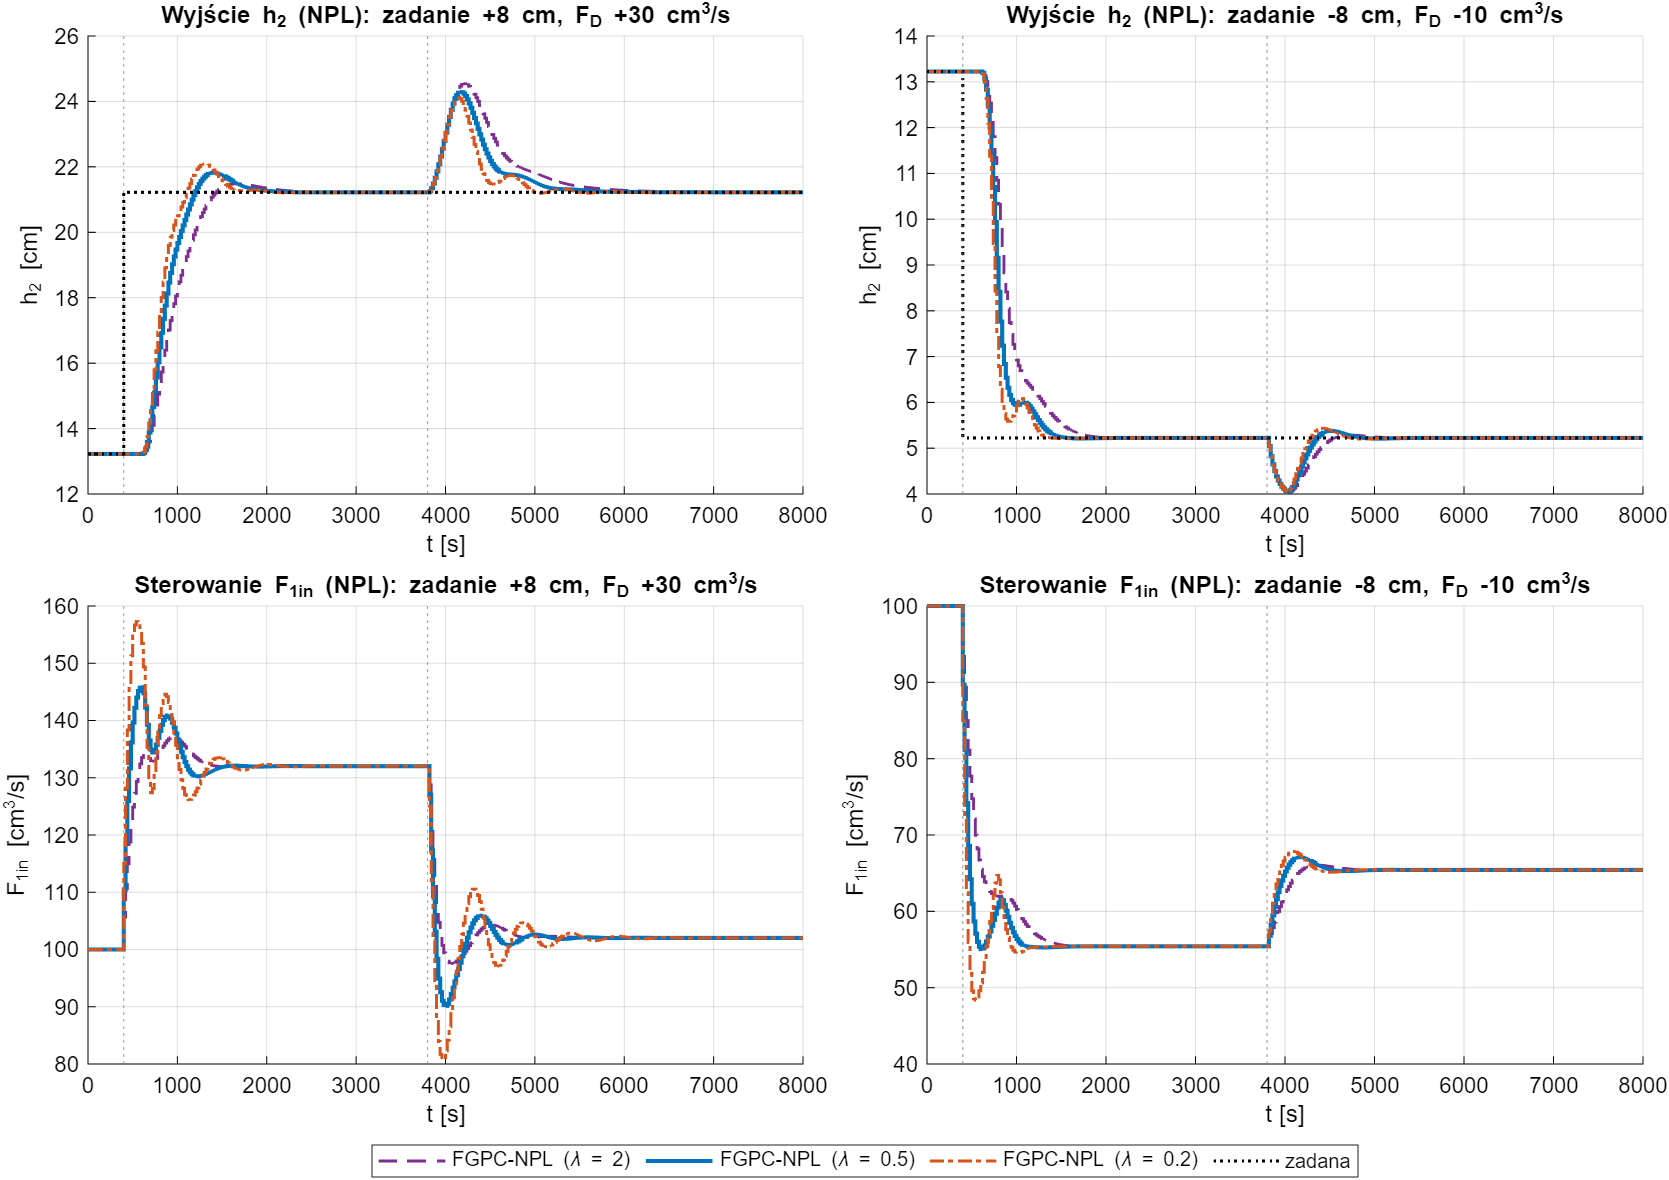
\includegraphics[width=\textwidth]{../wyniki_czesc4/strojenie_NPL.png}
\caption{Wpływ $\lambda$ na przebiegi $h_2$ i $\uvar$ w regulatorze FGPC--NPL (${N=30}$, ${N_u=5}$).}
\label{fig:npl-tuning}
\end{figure}
\begin{figure}[H]
\centering
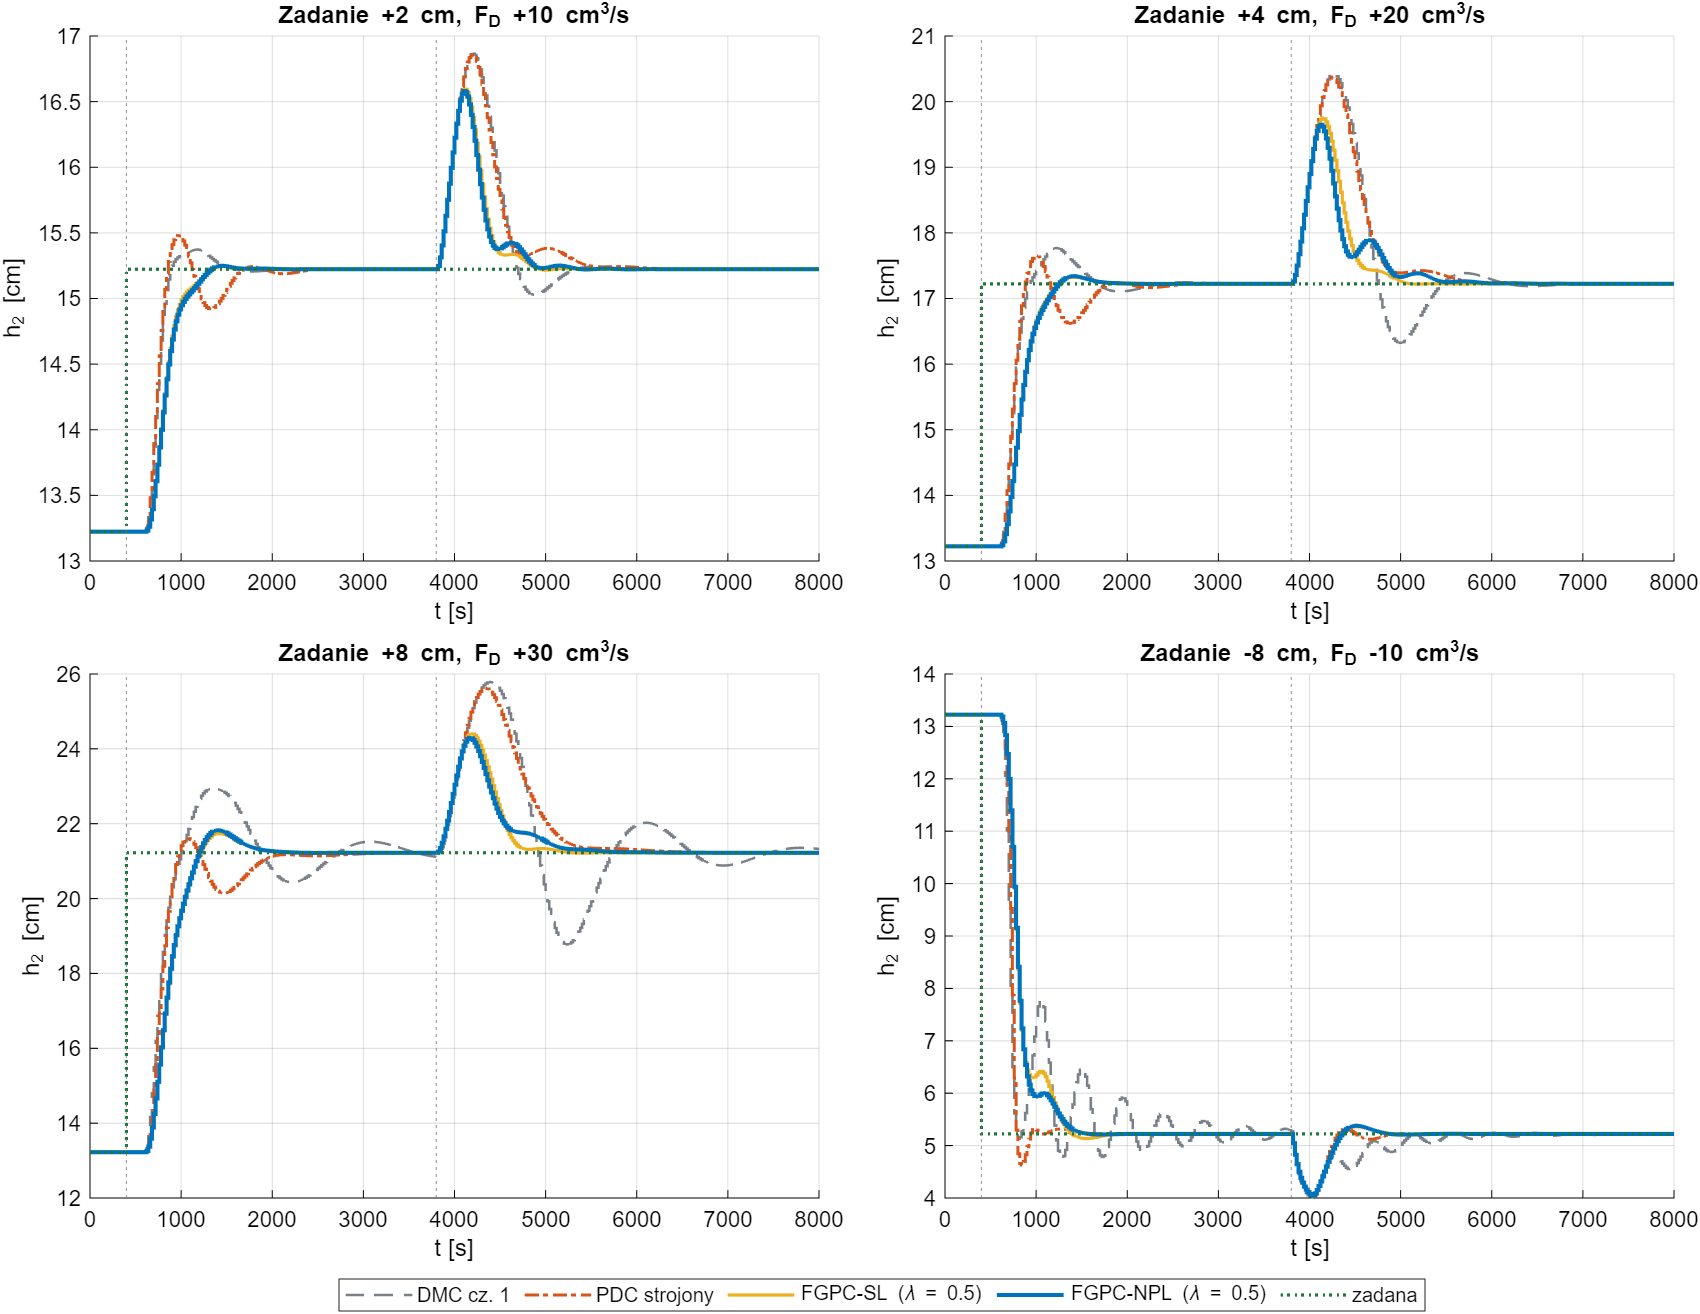
\includegraphics[width=\textwidth]{../wyniki_czesc4/NPL_y.png}
\caption{Poziom $h_2$ w czterech próbach: DMC z części~1, PDC strojony, FGPC--SL (${\lambda=\num{0.5}}$) i FGPC--NPL (${\lambda=\num{0.5}}$).}
\label{fig:npl-y}
\end{figure}
\begin{figure}[H]
\centering
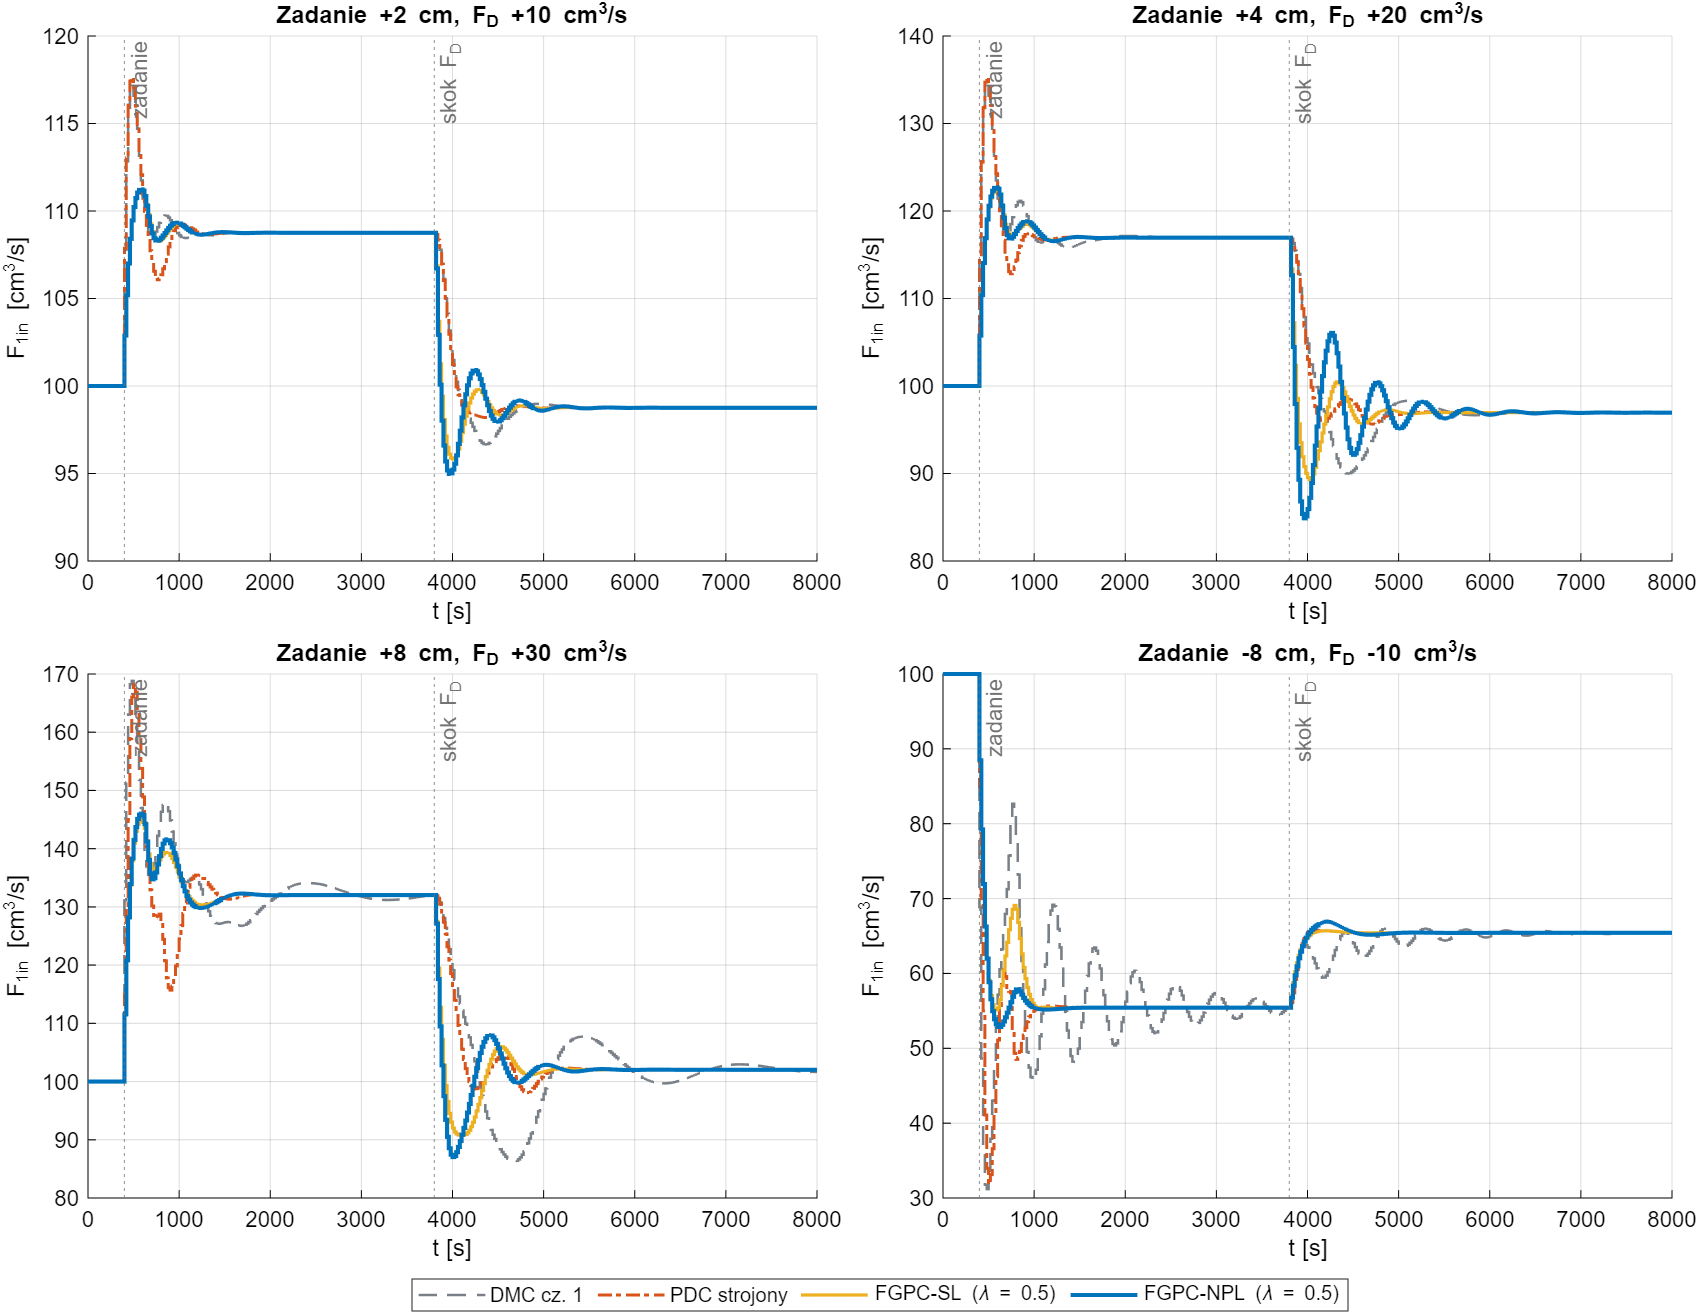
\includegraphics[width=\textwidth]{../wyniki_czesc4/NPL_u.png}
\caption{Sterowanie $\uvar$ dla przebiegów z rys.~\ref{fig:npl-y}.}
\label{fig:npl-u}
\end{figure}
